\documentclass[a4paper,10pt]{article}

% ---------- Packages ----------
\usepackage[a4paper,margin=1.5cm]{geometry}
\usepackage{paracol}          % two columns
\usepackage{tikz}             % graphics (photo circle + bars)
\usepackage{xcolor}
\usepackage{graphicx}
\usepackage{enumitem}
\usepackage[hidelinks]{hyperref}
\usepackage{fontawesome}      % reliable icons for pdfLaTeX (v4 set)
\usepackage{titlesec}

% ---------- Colors ----------
\definecolor{maincolor}{HTML}{D23F31}
\definecolor{textgray}{gray}{0.20}
\definecolor{barbg}{gray}{0.90}

% ---------- Spacing tweaks ----------
\setlength{\columnsep}{1.0cm}
\setlist[itemize]{noitemsep, topsep=1pt, leftmargin=1.2em}
\setlength{\parskip}{4pt}
\setlength{\parindent}{0pt}

% ---------- Language bar (0–5) ----------
\newcommand{\langbar}[1]{%
  \begin{tikzpicture}[baseline=-0.6ex]
    \fill[barbg]   (0,0) rectangle (5cm, 1.6pt);
    \pgfmathsetmacro{\w}{min(max(#1,0),5)*1.0} % clamp 0..5
    \fill[maincolor] (0,0) rectangle (\w cm, 1.6pt);
  \end{tikzpicture}%
}

% ---------- Section title ----------
\newcommand{\sect}[1]{\vspace{9pt}\textbf{\large #1}\vspace{-10pt}\par\textcolor{maincolor}{\rule{\linewidth}{0.8pt}}\vspace{4pt}}

\begin{document}\pagestyle{empty}\color{textgray}

% Control column widths (left:right)
\columnratio{0.36}
\begin{paracol}{2}

% ================= LEFT COLUMN =================
\begin{center}
  % Photo placeholder (circle)
  \begin{tikzpicture}
    %\draw[fill=barbg, draw=none] (0,0) circle (2.1cm);
    % Add your photo by replacing the fill with:
    \clip (0,0) circle (2.1cm);
    \node at (0,0) {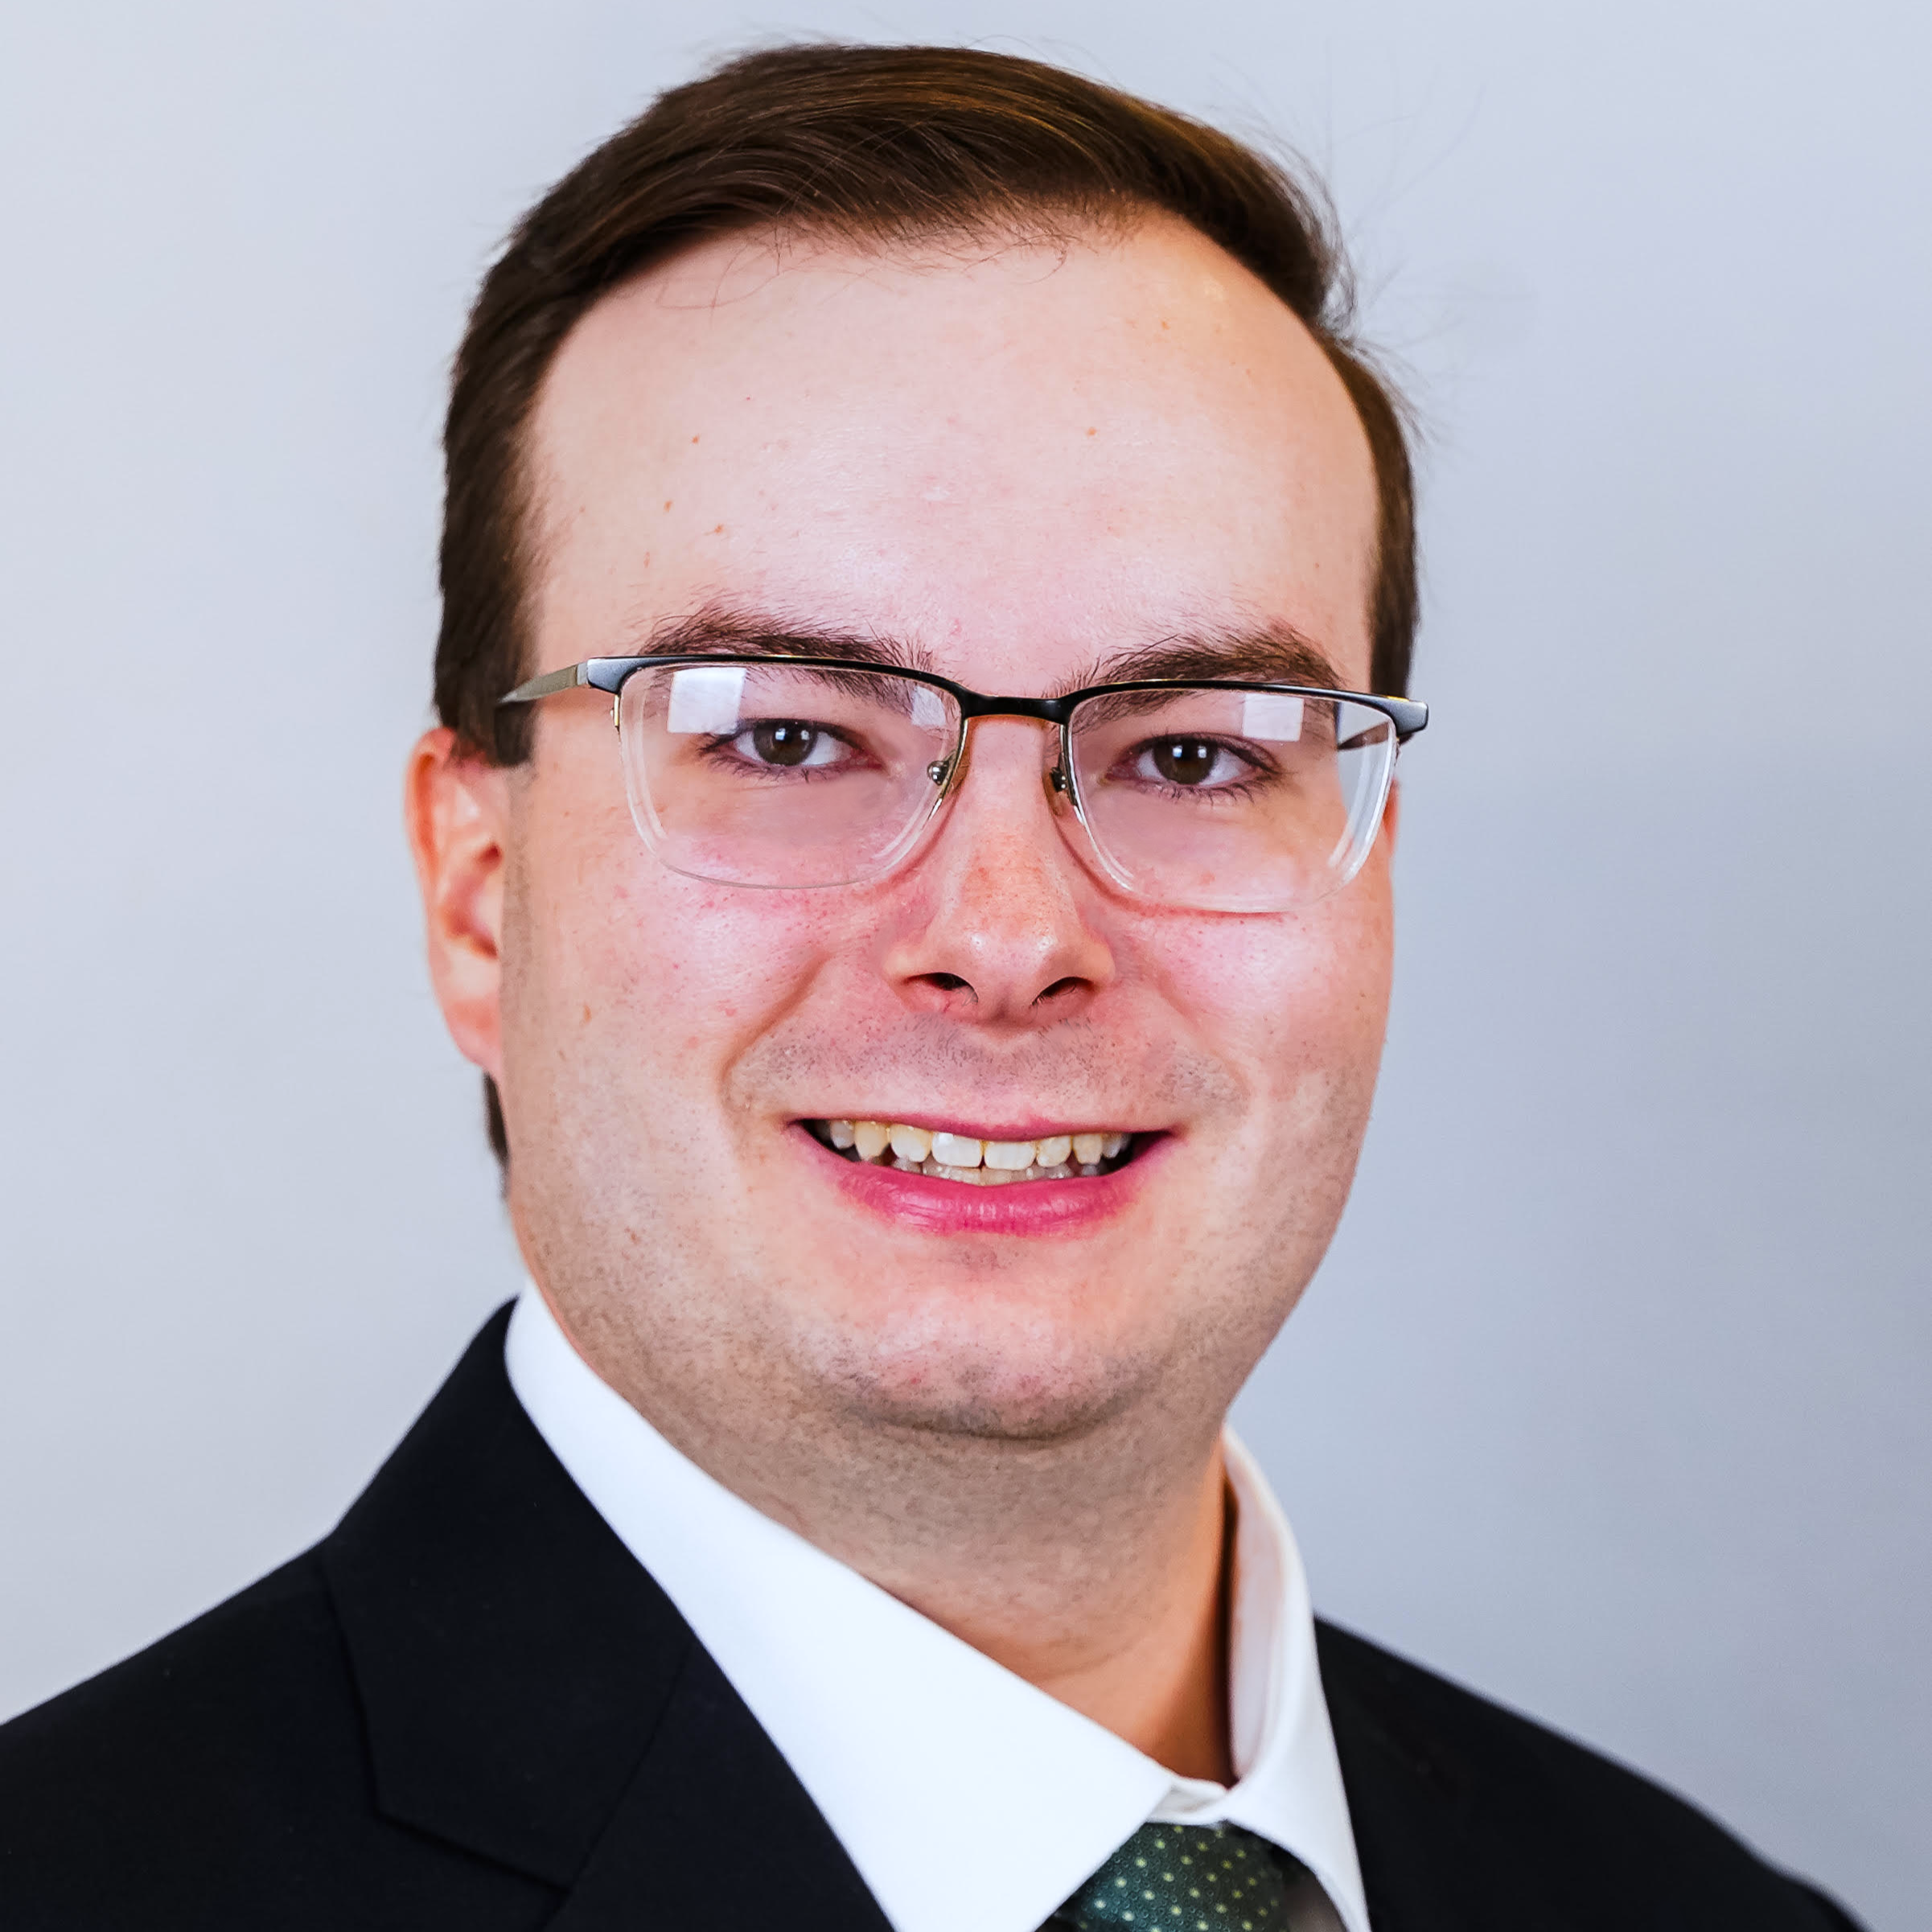
\includegraphics[width=4.2cm]{ColumHeadshot2_square.png}};
  \end{tikzpicture}

  \vspace{6pt}
  {\LARGE \textbf{Colum Cross}}\\[2pt]
  \textcolor{maincolor}{\rule{3.5cm}{1pt}}
\end{center}

\vspace{6pt}
\sect{Contact}
{\faPhone} ~ +1 (518) 956-3953\\
{\faPhone} ~ +49 162 8193963\\
{\faMapMarker} ~ Fischerinsel 15, 10179 Berlin\\
{\faEnvelopeO} ~ \href{mailto:columcross@gmail.com}{columcross@gmail.com}\\
{\faGlobe} ~ \href{http://columcross.com}{columcross.com}\\
{\faLinkedin} ~ \href{https://www.linkedin.com/in/columcross/}{linkedin.com/in/columcross}\\
{\faGithub} ~ \href{https://github.com/columcross}{github.com/columcross}\\

\sect{Languages}
\textbf{English} — Fluent\\
\textbf{German} — Conversational\par
\textbf{Programming Languages}
\begin{itemize}
    \item ServiceNow Developer: CSM, FSO, ITSM, SPM, Virtual Agent
    \item \textit{Frontend:} JS, Angular, React
    \item \textit{Backend:} Java, ColdFusion, PHP, Python
    \item \textit{Database:} MySQL, T-SQL, Oracle
    \item \textit{Mobile:} Java, Swift, C\#
\end{itemize}

\sect{Skills}
\begin{itemize}
    \item Proficient in ServiceNow platform development
    \item Front end and back end developer
    \item Mastery of Agile and Scrum Methodologies
    \item Experienced in end-user testing and usability research
\end{itemize}

\sect{Certifications}
\begin{itemize}
    \item ServiceNow Certified Application Developer
    \item ServiceNow Certified System Administrator
    \item Certified Lean Practitioner
\end{itemize}

\sect{Hobbies}
\begin{itemize}
    \item Travel
    \item Typewriter \& Watch Collecting
    \item Model Railroading
\end{itemize}

\switchcolumn

% ================= RIGHT COLUMN =================

\sect{Experience}

% === M&T ===
\textbf{Software Engineer II} \hfill M\&T Bank\\
2019 - 2025 \hfill \textit{Buffalo, New York}\par
\begin{itemize}
    \item Worked with stakeholders and Product Owners to prioritize work and understand business needs \& regulatory requirements
    \item Designed the look \& feel of ServiceNow applications
    \item Administered end-user testing to validate usability
    \item Core ServiceNow developer building required app functionality
    \item Solely developed an API and several integrations
    \item Lead manager responsible for pushing code to production
    \item Successfully converted several applications from the Update Set Model to the Application Publishing Model in ServiceNow
    \item Team lead on a project that researched solutions to address talent retention issues fit for a \$200B bank using the Desirability, Feasibility, Viability Model
    \item Volunteered with local schools to help teach programming to children in underserved communities
    \item Performed tech and behavioral interviews for Technology Development Program candidates
\end{itemize}
\medskip

% === RIT ===
\textbf{Web Developer} \hfill RIT Admissions\\
2018 \hfill \textit{Rochester, New York}\par
\begin{itemize}
    \item Frontend designer and developer for internal and external web applications
    \item Designed and developed an interactive kiosk for the lobby of the admissions department
\end{itemize}
\medskip

% === Ahold ===
\textbf{Web Developer} \hfill Ahold USA\\
2017 \hfill \textit{Quincy, Massachusetts}\par
\begin{itemize}
  \item Built a ColdFusion API for an Angular web app to aid local-produce ordering for store managers
  \item Developed an Angular app and ColdFusion API to manage company-wide email distribution
  \item Rebuilt a Java Web Pages backend in ColdFusion for large data volumes
\end{itemize}

\sect{Education}
\textbf{Rochester Institute of Technology}
\\ BS in Human-Centered Computing\par

\sect{Personal Projects}
\textbf{Permission Granted} \hfill \textit{Java for Android}\\	
An app for videographers, vloggers, and anyone who regularly uses release forms. Users are able to quickly and easily create, view, and sign release forms directly on their phone. Published on the Google Play Store.\par
\textbf{Warmer Colder} \hfill \textit{Java for Android}\\	
A two-player game based around your location. Uses the Android Location API to determine proximity to a location. Published on the Google Play Store.\par
\textbf{Tip Calculator for WearOS} \hfill \textit{Java for Android}\\
An application solely for Wear OS devices. It calculates a tip and total based on a base price and a tip percentage. Published on the Google Play Store.\par
\textbf{Math Based N-Back Test} \hfill \textit{C\# Universal Windows App}\\
An application that tests working memory by showing participants a series of single-digit math questions, then having them give the answer to the previous question. Published on the Windows Store.


\end{paracol}
\end{document}
